\documentclass[a4paper]{book} % If you don't know LaTeX, ignore everything until \begin{document}
\usepackage[utf8]{inputenc}
\usepackage{graphicx}
\usepackage{avant}
\renewcommand{\familydefault}{\sfdefault}
\addtolength{\evensidemargin}{-2cm}
\addtolength{\textwidth}{2cm}
\begin{document}
\fontsize{24}{28}\selectfont
\title{Introduction to Communism}
\author{Matvei "LeftHandedLeftist" Ivanov \\ and Kris Karlov}
\date{Written in 2018}
\maketitle
\fontsize{24}{28}\selectfont
\chapter{What is communism?}
Communism is a system where the means of production are owned by the community. The means of production are the tools that are needed to produce something. For example, machines in a factory are means of production.

It is different from the system most of the world has now. That system is called capitalism. It lets certain people or groups own the means of production while all other people work for them.

\begin{figure}[tbhp]
\centering
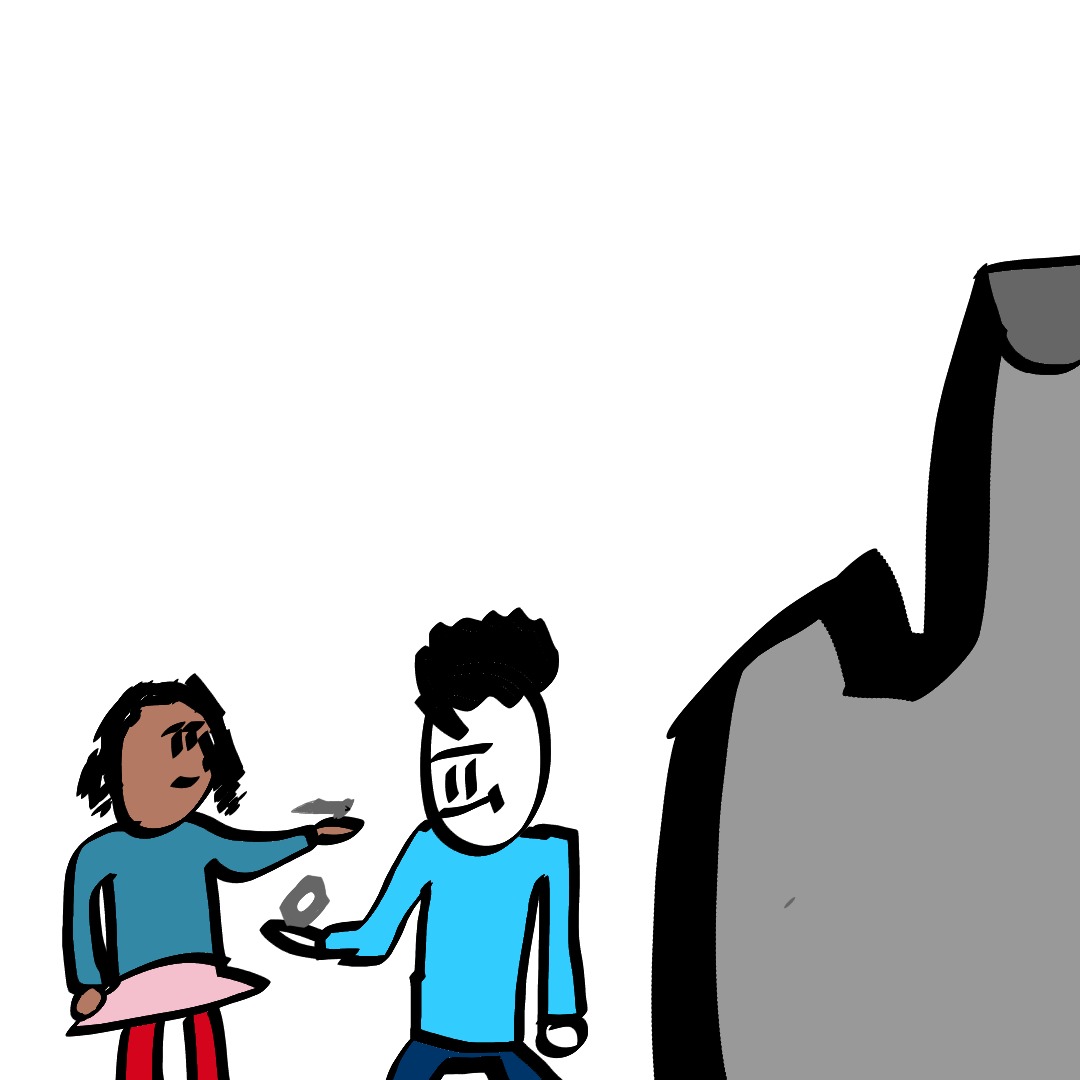
\includegraphics[width=0.9\textwidth]{1-1.png}
\caption{Under communism, the workers decide how much of what to produce}
\end{figure}

Because the owners the means of production under capitalism, who are also called the bourgeoisie, want to continue owning them, they often spread lies about what communism is and what happens while we get to it.

Often, they say that communism is when everyone owns everything. This is wrong. Only the means of production are owned by the community. The things that aren't used to produce something, also called personal property, can still be owned by a single person. Someone can still own a watch or a bicycle under communism. But the factories that produce watches or bicycles are owned by the community.

Sometimes they also call anything the state does communism. This is also wrong. Actually, there is no state under communism. It just isn't necessary. There are no reasons to fight about the means of production because they're already owned by everyone. And if someone wants to get them for themselves or starts a fight about personal property, the community will resist them.

Very often they say that communism is impossible, that humans will naturally try to get the most for themselves and only themselves. But they're wrong. Early humans did not have a single group owning the means of production. It was better for them to help their community, because they couldn't live without it: the community defended each other against the many dangers that were there.

\begin{figure}[tbhp]
\centering
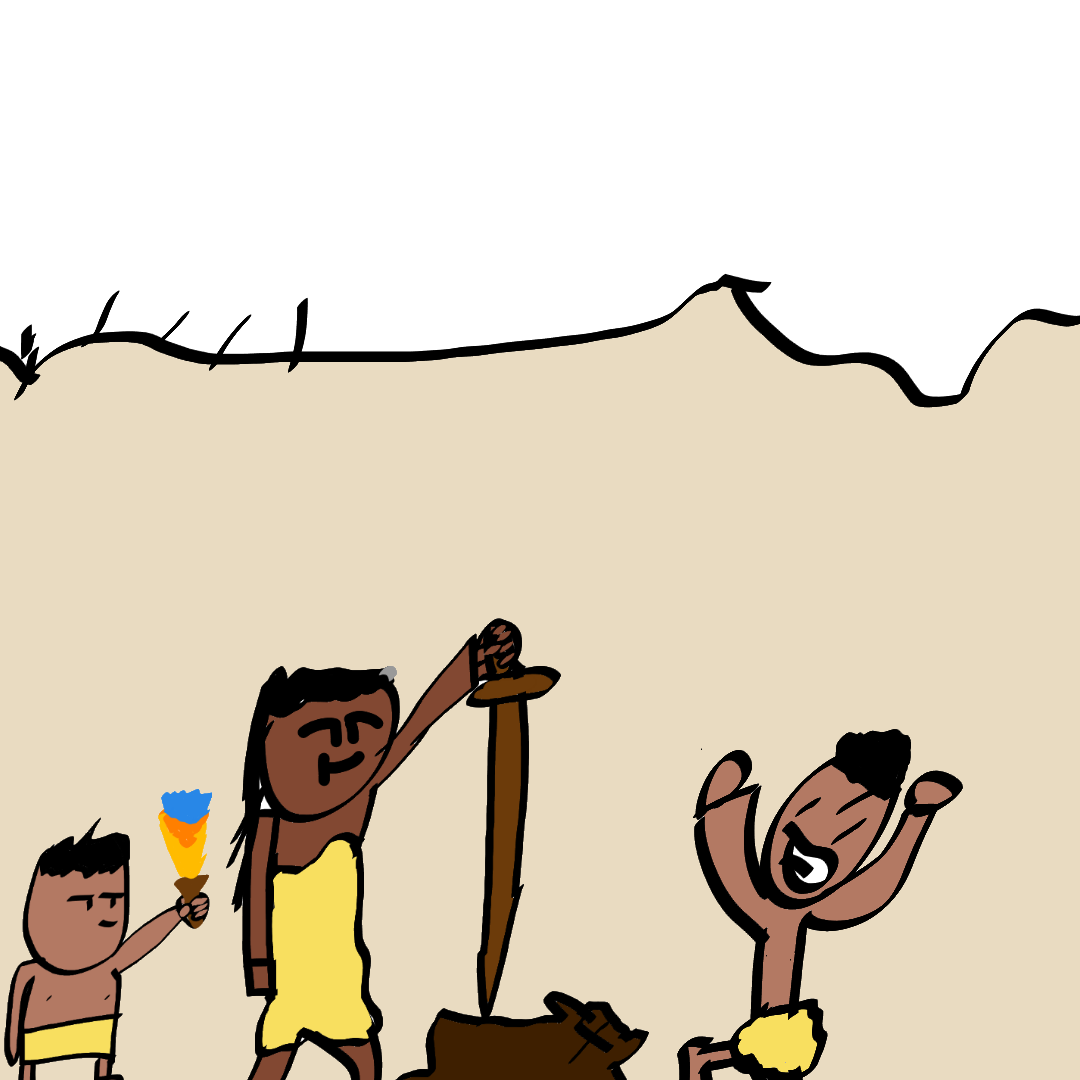
\includegraphics[width=0.9\textwidth]{1-2.png}
\caption{A group of early humans fighting a lion. Each of them couldn't do that alone, but in a strong community, they can.}
\end{figure}

Some say that the times have changed, the systems became more complicated, and communism can't exist now. It's true that it's not possible to immediately make a society communist now. This is why there is a step towards it called socialism. Socialism is possible, and it exists right now in a few countries.

\chapter{Why do we need communism?}

You see, the workers do almost all the work and the bourgeoisie do barely any. Even though the bourgeoisie does a small amount of work they get much much higher wages than the workers. We need to abolish (remove) this flaw. The best route is through SOCIALISM and COMMUNISM.

\begin{figure}[tbhp]
\centering
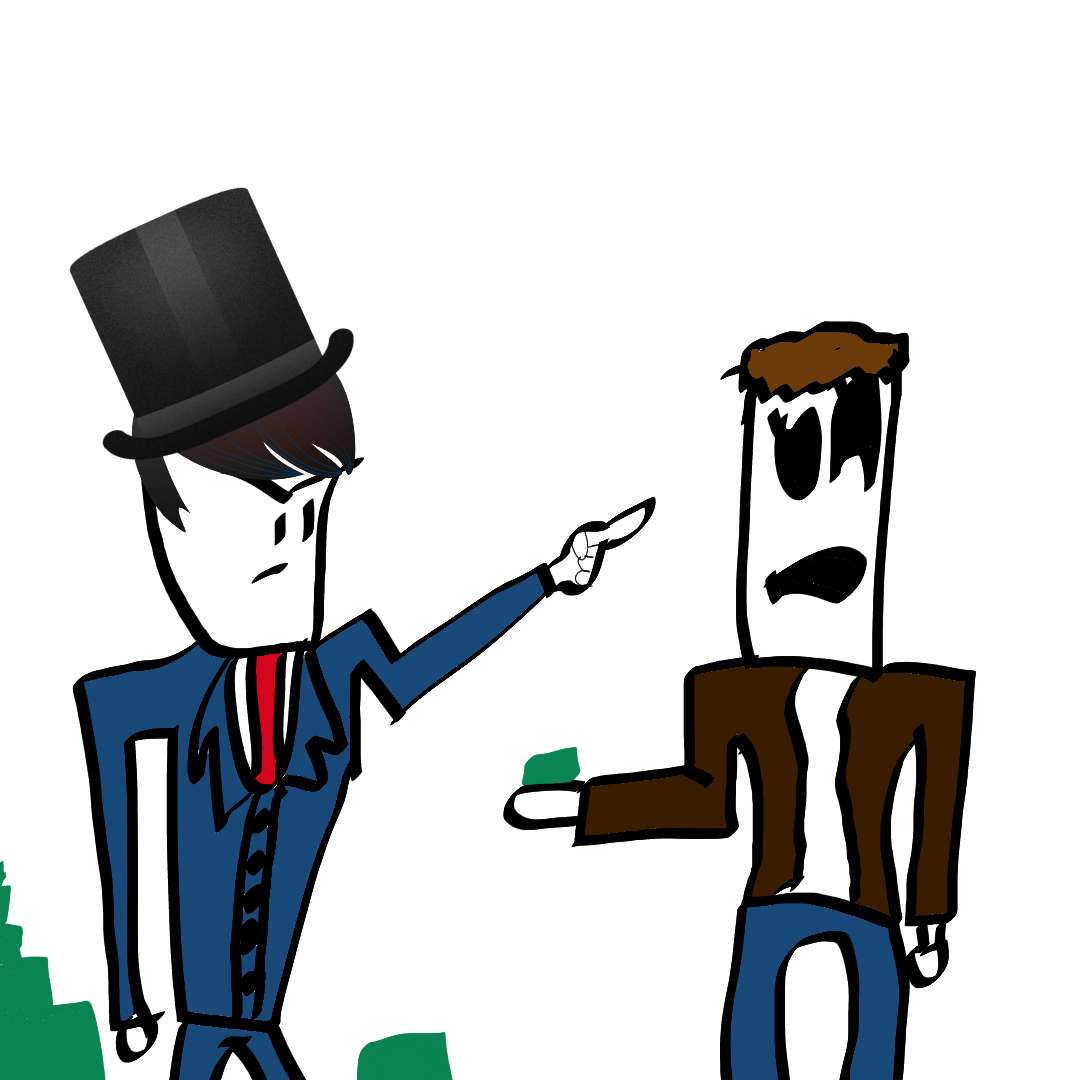
\includegraphics[width=0.9\textwidth]{2-1.png}
\caption{A bourgeois telling a worker where and how to work, while getting most of the money}
\end{figure}
  
  As we stated before, in communism the workers own the factories. Another great benefit of communism is the removal of money. This might sound silly; But you see, without money, there are no taxes and big projects (for example a new road) don't need money which means it can be done well and fast.

\begin{figure}[tbhp]
\centering
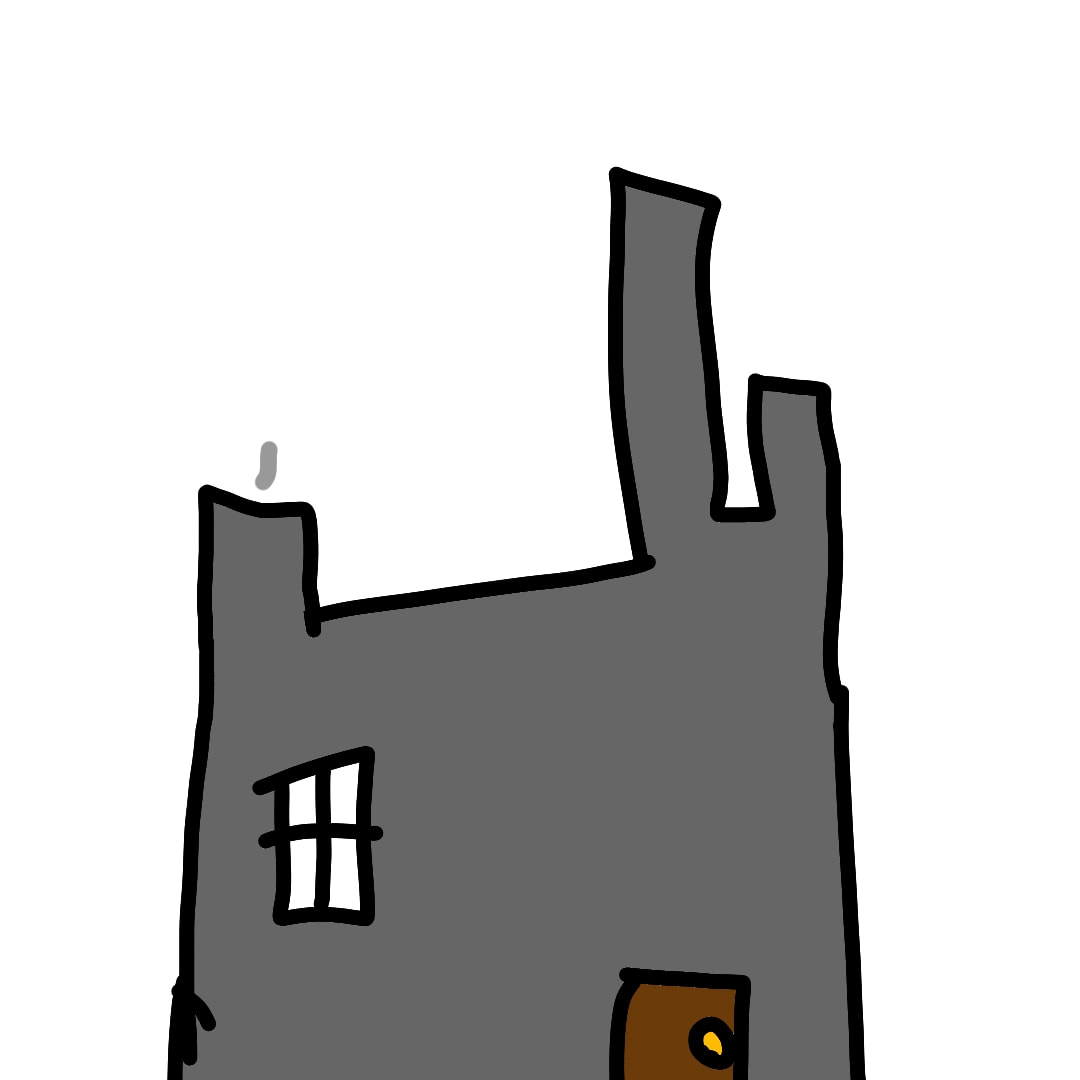
\includegraphics[width=0.9\textwidth]{2-3.png}
\caption{A factory, which is owned by the workers under communism and by the bourgeoisie under capitalism}
\end{figure}

  Under Communism, there is also no government. This is good because then the people must choose decisions.

\begin{figure}[tbhp]
\centering
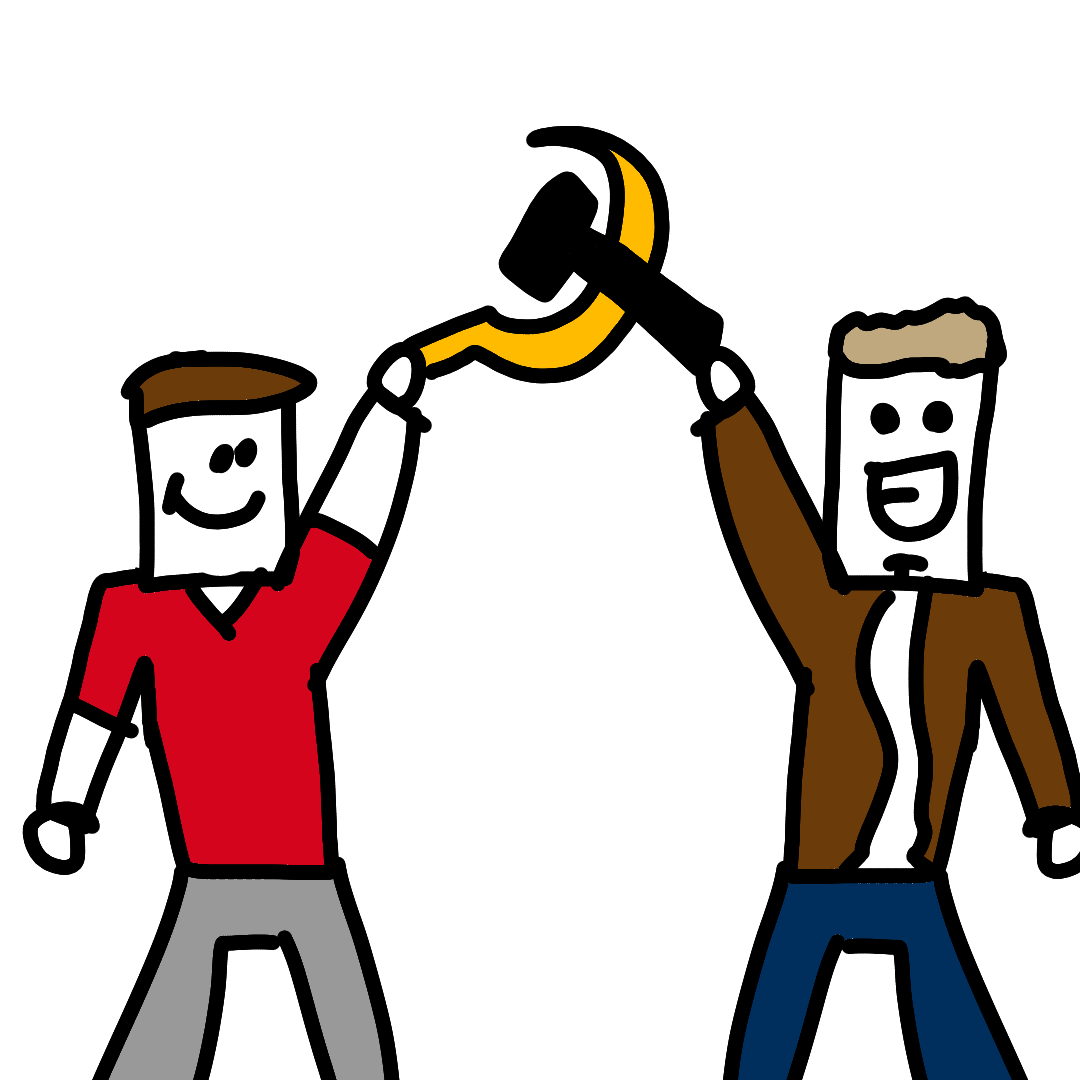
\includegraphics[width=0.9\textwidth]{2-5.png}
\caption{Under communism, the people themselves decide. So the decisions actually make the people happy, not some small group richer.}
\end{figure}

  Before COMMUNISM there should be Socialism. Socialism has a planned economy which means that random spikes in costs do not happen. Socialism does have money in its early stages; But after it has labour vouchers. 

\begin{figure}[tbhp]
\centering
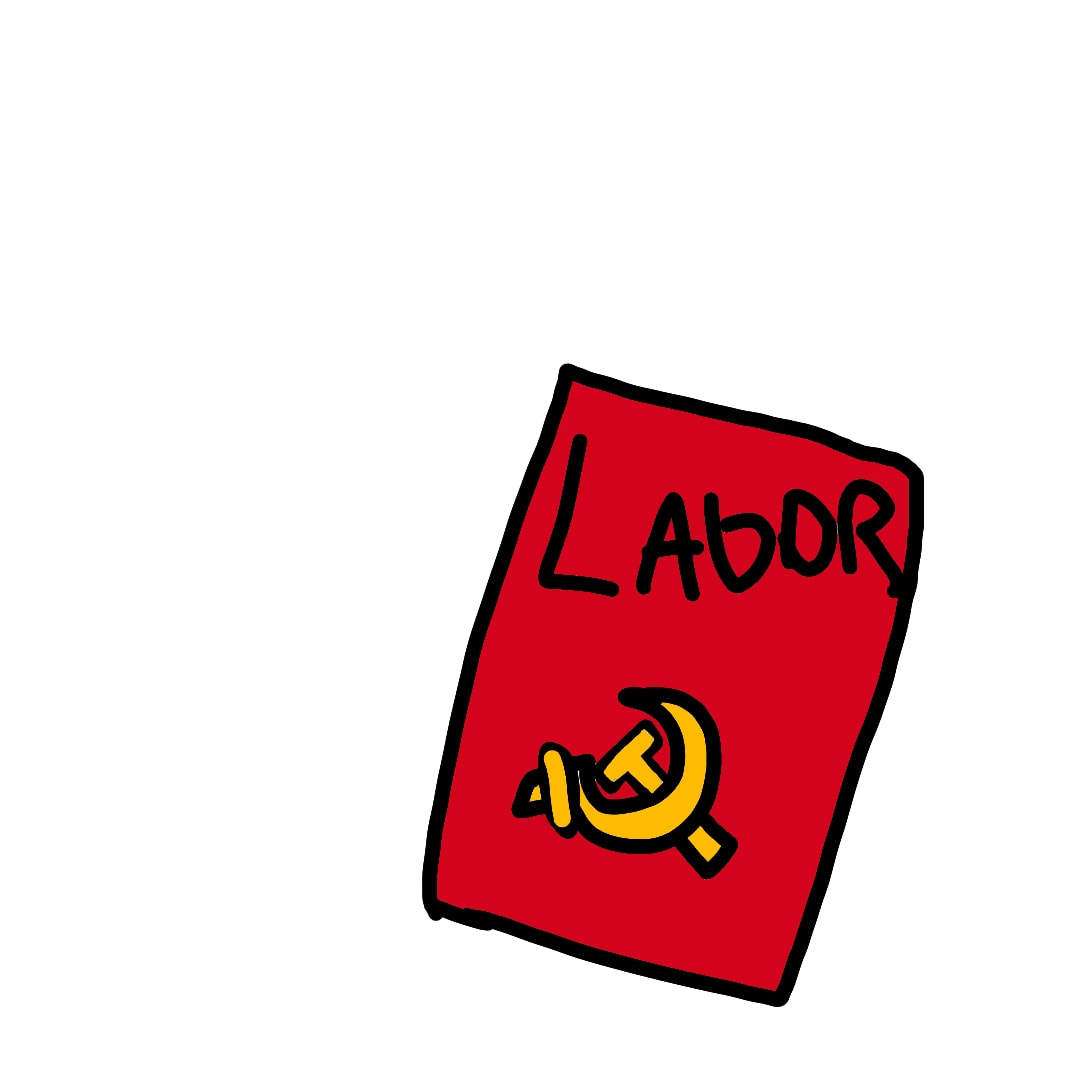
\includegraphics[width=0.9\textwidth]{2-4.png}
\caption{A labour voucher}
\end{figure}

  Labour vouchers are money that disappears after it is spent. This is so that people cannot make things extremely expensive and get huge profits. We might discuss this more in a later paper.

\chapter{How do we get to communism?}

The best route into communism is (sadly) violent.

The party usually stages a revolution that stops the current capitalist government and replaces it with a socialist one. Socialism is the step before communism.

\begin{figure}[tbhp]
\centering
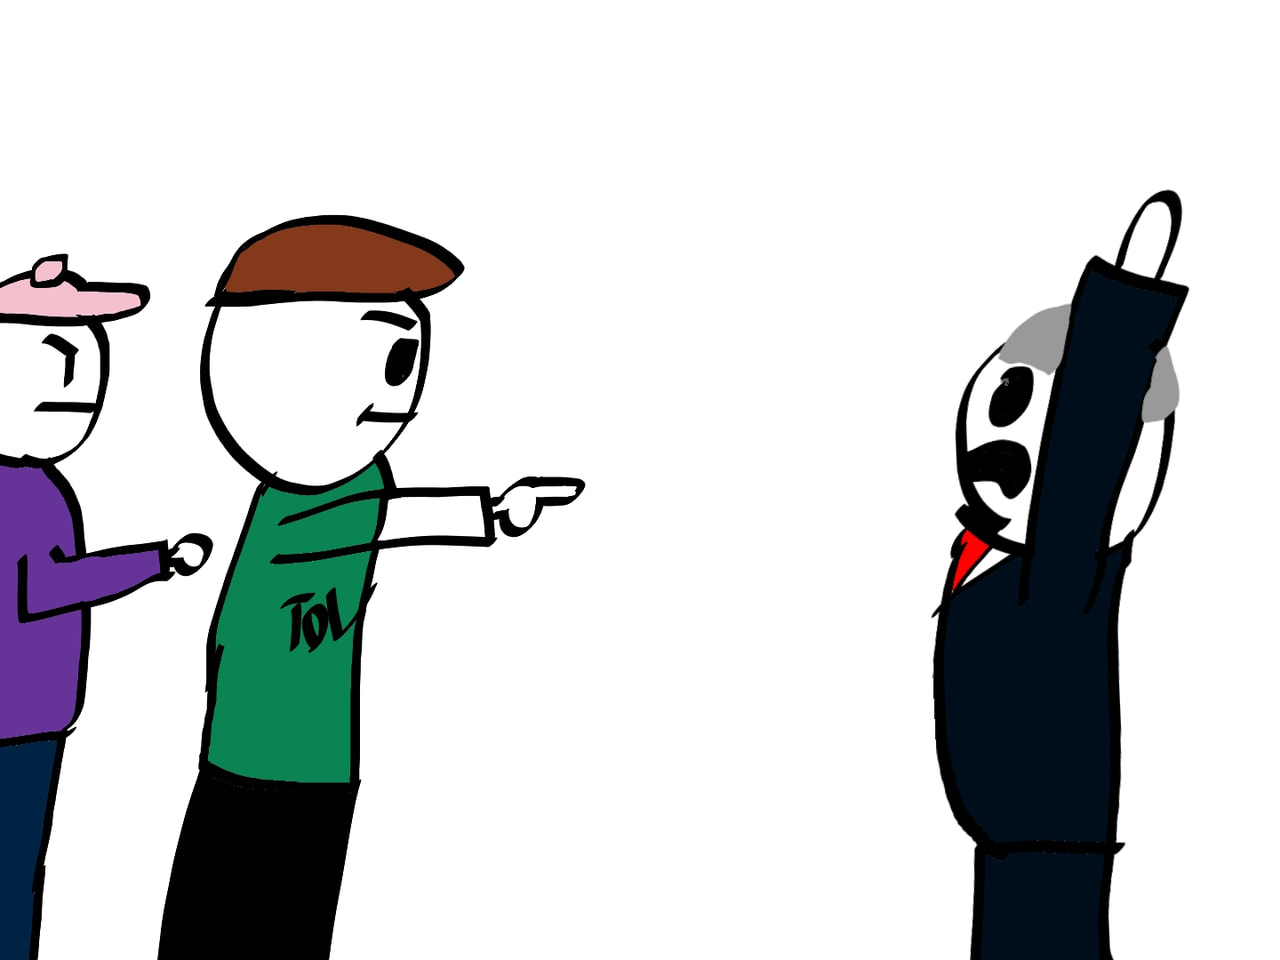
\includegraphics[height=0.3\textheight]{3-1.png}
\caption{Two revolutionaries attacking a capitalist}
\end{figure}

\newpage

Under socialism, the people and the government do communist reforms that make the country get closer to communism. In socialism, the government slowly fades away into communism. Socialism still has a government.

But the socialist government is different from a capitalist one. It doesn't allow a single person to own means of production. So the government gets the money that the owners of the means of production get under capitalism. It then uses that money for projects like a new road and for paying those who can't work, for example old people. Such a government doesn't need taxes anymore. That's why many socialist countries, for example Albania and the DPR Korea, abolished taxes.

\begin{figure}[tbhp]
\centering
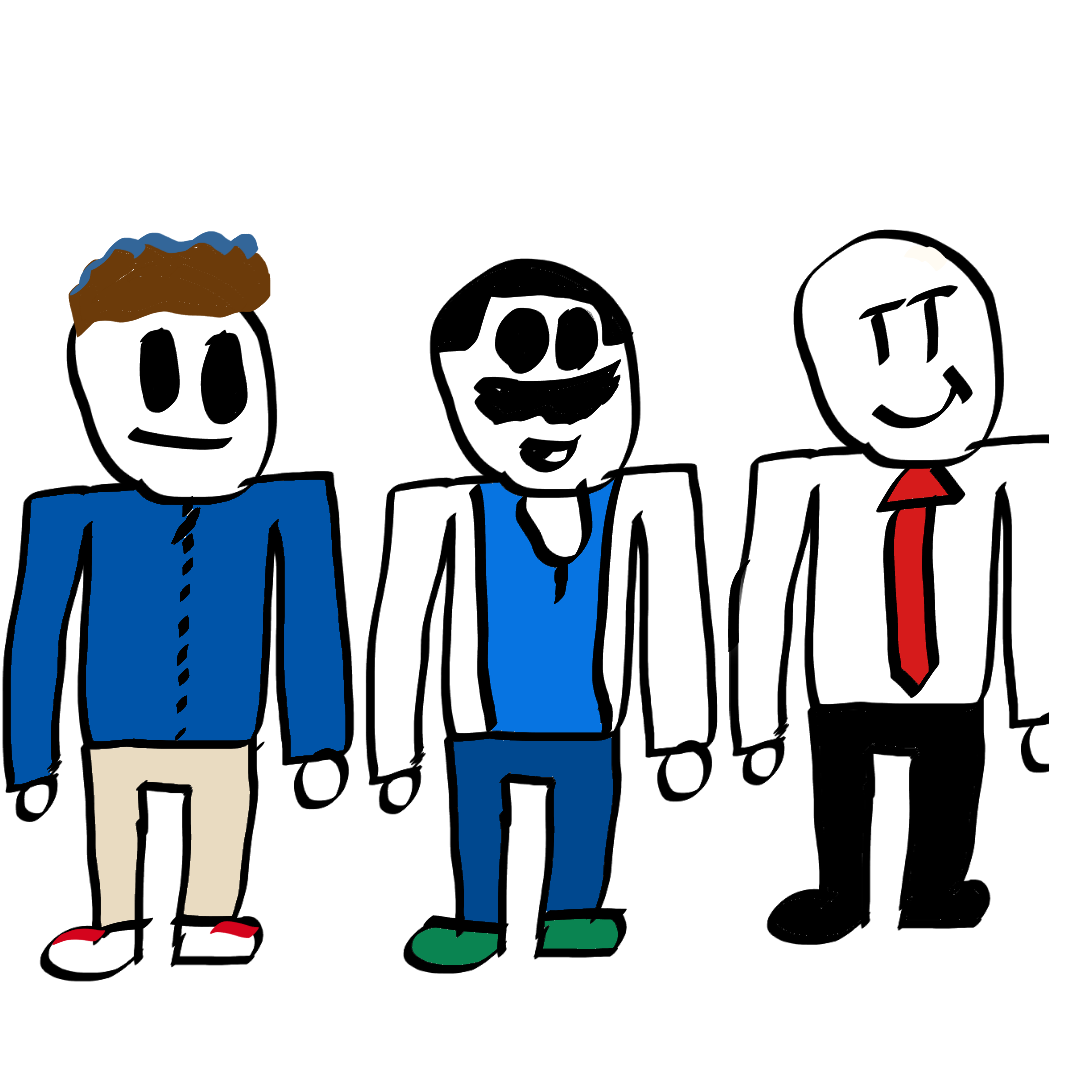
\includegraphics[width=0.9\textwidth]{3-2.png}
\caption{Three workers, who live better under socialism than under capitalism}
\end{figure}

The reason we need socialism and we can't skip straight to communism? It is because opposing forces (capitalists) can easily stop the land. Going straight to communism (anarchy) has been successfully done once before without falling in Africa. It survives because no one wants it to fall.

For communism to start you need world socialism.

\begin{figure}[tbhp]
\centering
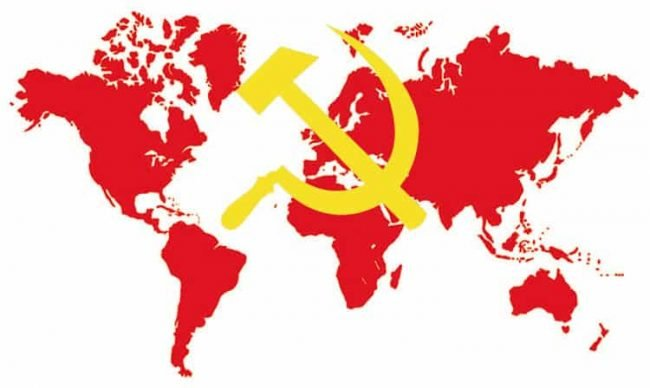
\includegraphics[width=0.9\textwidth]{3-3.jpg}
\caption{A socialist world}
\end{figure}

Once the socialist government is no longer needed and falls, full communism starts.

That's how we get into communism!

\chapter{Notable communists and their tendencies}

All over the world there were and are communists. Because there are differences between various countries, communism and socialism can't be the same everywhere. Also, communists think differently on what is most important for building communism. This is why there are various tendencies. This chapter will be about the most important tendencies and their supporters.

\section{Marxism --- Karl Marx and Friedrich Engels}

Karl Marx and Friedrich Engels lived in the 19$^{th}$ century, when capitalism just started developing. They looked at how capitalism worked and saw the many problems it brings. So they proposed another system, communism.

Although communism existed long before Marx and Engels, they were the first who wrote about what exactly communism is and how it will happen. While they did not fight for communism themselves, they helped organize the parties that did and criticized the ones that did it wrong.

Most communists' ideas rely on Marx's and Engels's theories, also called Marxism. This is why those who want us to believe that communism is wrong often tell us that Marx and Engels are wrong.

\section{Marxism-Leninism --- Wladimir Lenin and Josif Stalin}

Wladimir Lenin led the first successful communist revolution in 1917, which resulted in a socialist Soviet Union. Because the capitalist world didn't want Soviet socialism, they invaded it and tried to stop it. But the Soviet communists successfully resisted that invasion and started building socialism.

Lenin wrote a lot about what exactly must happen during and after the revolution. But he also looked at capitalism. While Marx saw only the initial stage of capitalism and could only predict what would happen later, Lenin saw how it developed and that Marx was right with these predictions.

He called the new stage of capitalism imperialism. Under imperialism, not only the means of production are in the hands of a few people, but also most of the money is in a few countries. These countries build roads, buildings and other useful things everywhere else, but only to get ressources for themselves, not to help anyone living there.

Because it also gets money and resources from the rest of the world, not only its own country, the bourgeoisie of these few countries can let some workers live well. This often makes these workers ignore that capitalist problems because they're not affected much by them. The bourgeoisie then tells us that anyone can be like these workers, making revolution even more difficult.

Josif Stalin didn't have many new ideas. But he led Soviet socialism to success using the Marxist-Leninist theories.

Stalin's government is often criticized for being too violent. But violence was necessary to resist the constant attacks on the Soviet Union from outside. Because when its capitalist enemies could no longer directly invade it, they tried destroying the Soviet Union from inside. And there were enemies of communism in the Soviet Union itself, too.

With Stalin leading the Soviet Union, it also won a war against the German fascists, which were invading most of Europe. Although the USA and the UK helped the Soviet Union later in that war, it achieved an important victory in 1942 without help from outside. This victory stopped the German invasion and let the Soviets invade Germany instead.

\end{document}
